% Paper 3: Three-figure scientific review release (2026-10-10).
% Uses the archived batch20 integrity-correction replication.
% Source figures are embedded unchanged; see FINAL_SCIENTIFIC_REVIEW.md.
% Author metadata and Fig.1 RI branch arrow require author sign-off before submission.
\documentclass[journal]{IEEEtran}
\usepackage{amsmath,amssymb}
\usepackage{algorithm,algpseudocode}
\usepackage{booktabs,multirow,array,graphicx,url,microtype,enumitem}
\usepackage{hyperref,placeins}
\setlist[itemize]{leftmargin=*,nosep}
\hypersetup{hidelinks}
\title{Bounded Maintenance Recoverability for Selective Lifecycle Escalation of Digital-Twin Models}
\author{Author metadata to be confirmed before submission}
\begin{document}
\maketitle
\begin{abstract}
A deployed digital-twin (DT) model is commonly maintained through repeated parameter-level adaptation as operating conditions evolve. This strategy implicitly assumes that the current model identity remains suitable and that local maintenance can recover acceptable service quality. That assumption can fail under persistent regime shifts or structural mismatch, where continued adaptation yields limited benefit and model-level re-instantiation becomes a relevant lifecycle option. This paper formulates \emph{bounded fixed-identity maintenance recoverability}, which asks whether an admissible fixed-identity maintenance policy can achieve average service loss at or below a specified threshold over a given horizon and within a maintenance budget. Because future recoverability cannot be observed at decision time, a frozen estimator produces a recoverability-related admission score from causal, identity-normalized maintenance-response evidence, using supervision from finite one-shot maintenance references. A negative score admits model-level alternatives but does not force re-instantiation. Deployment-feasible alternatives then compete with retention and local maintenance under the same causal assessment data and frozen action costs. In an integrity-correction replication on 20 previously evaluated synthetic centers, the proposed policy has lower mean lifecycle service loss than frozen, unconditional-maintenance, and verification-guided local-maintenance baselines, with marginal 95\% paired center-bootstrap intervals for the differences below zero. Relative to always-open search, it admits model-level search at 33.30\% of stages and records 67.29\% fewer candidate-search optimizer updates. The observed service-loss difference relative to always-open search is small, with a confidence interval crossing zero; this does not establish equivalence or noninferiority. Offline diagnostics still expose substantial missed-escalation flags, limiting claims about escalation timing.
\end{abstract}
\begin{IEEEkeywords}
digital twin, lifecycle decision, recoverability, continual maintenance, model identity, re-instantiation, deployment constraints
\end{IEEEkeywords}

\section{Introduction}
\label{sec:intro}
Deployed digital-twin (DT) models in computing and networked infrastructures must remain useful as workloads and operating conditions evolve \cite{Sharma2022,Mihai2022,Xu2023,Tang2022,Qin2024}. A common response is to adapt the parameters of the deployed model using newly available observations \cite{Tao2026,Luo2025,Wang2024CL}. This preserves its model identity and can be effective when its learned representation remains suitable. However, a successful update at one stage does not establish that the same identity can maintain an acceptable service level over a longer horizon under limited adaptation effort. With sustained regime changes or structural mismatch, additional parameter updates may provide insufficient recovery, making a different model identity a relevant lifecycle alternative.

This distinction exposes a decision problem not resolved by drift detection or adaptation triggers alone \cite{Zhang2023OneNet,Kim2022RevIN,Liu2022NST}. Detecting a distributional change does not determine whether the current identity can meet a service requirement under a bounded maintenance policy; nor does a limited response to an individual update establish that no feasible maintenance policy remains. We therefore examine \emph{bounded fixed-identity maintenance recoverability}: whether an admissible maintenance policy can achieve average service loss no greater than a specified threshold within a given horizon and maintenance budget, without changing model identity. Because this quantity depends on future service outcomes, it cannot be evaluated directly at online decision time. Evidence suggesting insufficient recoverability may justify \emph{admitting} model-level alternatives, but does not by itself justify \emph{committing} to a different identity. The latter decision still requires comparison with retention and local maintenance.

We address this lifecycle decision through causal maintenance-response evidence and selective model-level search. At each stage, a bounded probe assesses the response of the current identity to local adaptation without immediately replacing the deployed parameters. Trained on offline targets constructed from finite one-shot maintenance references, a frozen estimator produces a recoverability-related admission score from causal, identity-normalized response history. A negative score opens access to deployment-feasible model-bank alternatives; otherwise, the controller considers retention and local maintenance only. When search is admitted, eligible actions are compared on available assessment data under a frozen loss-plus-penalty rule. Only the selected action is committed, and re-instantiation resets identity-specific evidence. This separates \emph{whether to consider} a different identity from \emph{whether to deploy} it.

The main contributions are as follows:
\begin{itemize}
\item \textbf{Bounded fixed-identity maintenance recoverability.} We formulate a lifecycle-level criterion under a service threshold, maintenance horizon, budget, and admissible fixed-identity policy class. The definition distinguishes the sufficiency of continued parameter-level maintenance from the availability of model-level alternatives.
\item \textbf{Maintenance-response-based admission evidence.} We construct causal, identity-normalized maintenance-response features and train an estimator using finite one-shot maintenance references. Once frozen, the estimator produces an imperfect online admission score rather than a direct evaluation of full-class recoverability.
\item \textbf{Selective lifecycle escalation.} We use the score to conditionally admit deployment-feasible re-instantiation candidates while retaining local maintenance and retention as competing actions. Assessment-based action comparison determines whether an identity change is committed; identity-specific evidence is reset only after re-instantiation.
\end{itemize}

\section{Related Work}
\label{sec:related}
\subsection{Digital-Twin Lifecycle and Continual Maintenance}
Recent DT surveys describe lifecycle synchronization, heterogeneous sensing, network-level virtualization, and model updating as central engineering challenges \cite{Sharma2022,Mihai2022,Xu2023,Tang2022,Qin2024}. In edge environments, EDT-SaFL investigates semi-asynchronous federated training \cite{Tao2026}, whereas personalized federated learning supports DT construction and transfer across social IoT nodes \cite{Luo2025}. These approaches address model learning and updates. Continual learning studies sequential knowledge retention \cite{Wang2024CL}. At test time, CoTTA smooths adaptation through teacher and prediction averaging, whereas EATA filters uninformative updates and mitigates forgetting \cite{Wang2022CoTTA,Niu2022EATA}. RoTTA, EcoTTA, and SAR target streaming correlation, memory costs, and stability under dynamic changes, respectively \cite{Yuan2023RoTTA,Song2023EcoTTA,Niu2023SAR}. More recent CTTA work explores representation learning, adaptive supervision, and prompt-based updating \cite{Liu2024MAE,Yang2024CTTA,Chen2024VPTTA}. These studies demonstrate that maintaining changing models is an established research problem; the present work does not claim to introduce post-deployment updating or selective adaptation. Instead, it asks whether the \emph{current model identity} can satisfy a future service threshold under bounded maintenance, and uses evidence about that question to regulate access to alternative identities.

\subsection{Drift Detection and Adaptation Decisions}
Online learning and forecasting research directly addresses nonstationarity. OneNet adjusts an ensemble under streaming concept drift \cite{Zhang2023OneNet}, while RevIN and Non-stationary Transformers address distributional changes in time-series forecasting \cite{Kim2022RevIN,Liu2022NST}. PatchTST provides an alternative forecasting representation and demonstrates transferable pretraining \cite{Nie2023PatchTST}. These methods make forecasting more adaptive or accurate, but neither a change indicator nor a one-stage prediction improvement establishes the best horizon-averaged service quality achievable by bounded maintenance of a fixed deployed identity. Importantly, this distinction is conceptual rather than a claim that drift-aware methods cannot change models or adapt model ensembles. Our recoverability criterion refers to a future maintenance-policy class, while the implemented admission score is a supervised proxy obtained from a finite one-shot policy subset.

\subsection{Model Selection, Switching, and Re-instantiation}
Resource-aware model design and deployment already address architectural alternatives and operational constraints. Surveys of end--edge--cloud computing discuss heterogeneous deployment trade-offs \cite{Wang2024EndEdge}; EfficientFormer and EfficientFormerV2 construct efficient model families under latency and model-size considerations \cite{Li2022EfficientFormer,Li2023EfficientFormerV2}. MCUNetV2 jointly explores neural designs and inference schedules for limited device memory \cite{Lin2021MCUNetV2}. Such work establishes constrained model selection and hardware-aware design as prior capabilities. Our contribution is not a novel model bank, neural architecture search operator, or proof that model switching was previously absent. Instead, we study a separate \emph{post-deployment admission condition}: whether the response of the currently deployed identity to bounded maintenance warrants considering source-initialized, deployment-feasible alternatives. After admission, retaining the deployed state and locally adapting it remain legitimate competitors. This formulation differs from initial few-shot model instantiation, which chooses an identity for a newly configured center, and from verification-guided fixed-identity maintenance, which decides whether to commit an adapted parameter state without introducing a different identity. Neither distinction implies that these earlier mechanisms were unavailable or ineffective.

\section{Problem Formulation}
\subsection{Lifecycle State and Causal Data}
At lifecycle stage $t$, let the deployed DT model state immediately
before the decision be
\begin{equation}
Z_t=(m_t,\theta_t),
\end{equation}
where $m_t$ denotes the model identity and $\theta_t$ its parameters.
This represents the deployed model, not the controller's complete
history-dependent state. Update data $D_t^{\mathrm{upd}}$ and assessment
data $D_t^{\mathrm{assess}}$ are visible to the online controller before
the action $a_t$ is selected. Current-stage service data
$D_t^{\mathrm{srv}}$ are withheld from the decision interface until
the action is committed and sealed. The causal order is
\begin{equation}
D_t^{\mathrm{upd}},D_t^{\mathrm{assess}}
\prec a_t\prec D_t^{\mathrm{srv}}.
\end{equation}
Past service observations may subsequently enter a later stage's
update data; the restriction concerns future information at the
current decision.

The available lifecycle actions are
\begin{equation}
a_t\in\{\mathrm{retain},\mathrm{maintain},\mathrm{reinstantiate}\}.
\end{equation}
Retention preserves the current model and parameters. Local maintenance
commits an adapted parameter state while retaining the model identity.
Re-instantiation may commit a different model identity and its adapted
parameters after candidate comparison. The selected action is
committed once to produce the next deployed state,
\begin{equation}
Z_{t+1}=\mathcal T_t(Z_t,a_t;D_t^{\mathrm{upd}},D_t^{\mathrm{assess}}).
\end{equation}
Stage-$t$ service is then evaluated using $Z_{t+1}$ on
$D_t^{\mathrm{srv}}$. The transition notation includes the applicable
frozen candidate construction and action-commitment rules.

\subsection{Bounded Fixed-Identity Maintenance Recoverability}
Let $H\in\mathbb N_{+}$ be a maintenance horizon and $B_M\geq0$ a
maintenance budget. Let $\mathcal A_M=\{\mathrm{retain},\mathrm{maintain}\}$
contain the fixed-identity actions. The admissible causal policy class is
\begin{equation}
\begin{aligned}
\Pi_t^M(H,B_M)=\bigl\{\pi:\;&
 m_{t+h}^{\pi}=m_t,\quad 1\le h\le H,\\
&\sum_{h=0}^{H-1}c_M(a_{t+h}^{\pi})\le B_M
\bigr\},
\end{aligned}
\end{equation}
where $a_{t+h}^{\pi}\in\mathcal A_M$, $c_M$ measures maintenance
expenditure, and $c_M(\mathrm{retain})=0$.
Each policy observes only the information available by its decision
time. For $\pi\in\Pi_t^M(H,B_M)$, define the horizon-averaged
service loss
\begin{equation}
\mathcal J_t^M(\pi;H)=\frac1H\sum_{h=0}^{H-1}
\mathcal L_{t+h}^{\mathrm{srv}}
(m_t,\theta_{t+h+1}^{\pi}).
\end{equation}
Given a service-loss threshold $\tau_{\mathrm{svc}}$, bounded
fixed-identity maintenance recoverability is
\begin{equation}
\mathcal R_t^M(H,B_M)=\tau_{\mathrm{svc}}-
\inf_{\pi\in\Pi_t^M(H,B_M)}\mathcal J_t^M(\pi;H).
\end{equation}
A positive value implies that some admissible policy achieves
average service loss below the threshold. A negative value means
that no policy in the specified class reaches the threshold.
At equality, a feasible policy must attain the infimum for
recoverability to hold.

This definition is conditional on the policy class, horizon,
budget, and threshold. A finite subset
$\widehat\Pi_t^M\subseteq\Pi_t^M$ can provide a restricted
hindsight reference, but failing to reach the threshold within
that subset does not establish unrecoverability over the full
class. The evaluation below does not solve the full dynamic
policy-class infimum.

\subsection{Online Decision Problem}
The future-dependent theoretical quantity $\mathcal R_t^M$ is
unavailable at decision time. The implemented controller instead
uses a causal, recoverability-related admission score $q_t$.
This score is supervised by a finite-policy reference defined
in Section~IV-B; it is not a numerical observation or calibrated
estimate of the full-class $\mathcal R_t^M$. Its frozen
admission rule is
\begin{equation}
q_t\geq0\ \Rightarrow\ \text{model-level search closed},
\end{equation}
\begin{equation}
q_t<0\ \Rightarrow\ \text{model-level search admissible}.
\end{equation}
The decision signal is fallible: admitting model-level search
does not prove that fixed-identity maintenance is impossible,
and opening the gate does not force re-instantiation.

\section{Recoverability-Guided Lifecycle Method}
\subsection{Bounded Local-Maintenance Probe}
At stage $t$, a provisional maintenance candidate is obtained
by applying 50 optimizer updates to a copy of the deployed
parameters using $D_t^{\mathrm{upd}}$. The deployed parent remains
unchanged until action commitment. Let $\ell_t^{\mathrm{pre}}$
and $\ell_t^{\mathrm{post}}$ be the losses of the parent and
provisional candidate on the same $D_t^{\mathrm{assess}}$.
The relative maintenance gain is
\begin{equation}
g_t=\frac{\ell_t^{\mathrm{pre}}-\ell_t^{\mathrm{post}}}
{\ell_t^{\mathrm{pre}}+10^{-12}}.
\end{equation}
This probe supplies an assessment-based response event even when
the eventual action is retention. Events are stored only within
the current model-identity lifetime and cleared when a different
identity is committed.

\subsection{Identity-Normalized Recoverability Evidence}
For each model-identity lifetime, define the positive reference scale
\begin{equation}
S_m=\max\!\left\{\operatorname{median}(e_1,\ldots,e_{104}),
10^{-12}\right\},
\end{equation}
where a causal reference segment of 200 raw observations produces
104 pointwise squared errors after the 96-observation input context.
At initial deployment, this reference is taken from the frozen
post-warm-up segment. Following re-instantiation, it is rebuilt
using the newly selected model and the last 200 raw observations
of the current assessment segment. The scale is held fixed for
the resulting identity lifetime.

The current response event contains $g_t$ and the normalized
post-probe residual $r_t=\ell_t^{\mathrm{post}}/S_m$.
Including the current event, short and long history lengths
$K_S=2$ and $K_L=6$ form the six features
\begin{equation}
\boldsymbol x_t=(\bar g_S,\bar r_S,\bar g_L,\bar r_L,
n_S/2,n_L/6).
\end{equation}
Here the bars denote means over the available events within
each window, and $n_S,n_L$ are their counts. Features are
standardized using fitting-only statistics. A frozen MLP with
architecture $6\!\rightarrow\!16\!\rightarrow\!8\!\rightarrow\!1$
(two ReLU hidden layers and a linear output) produces the online
admission score $q_t$.

The score has explicit but limited supervision. The theoretical
policy-class quantity is not directly used as a training target;
we instead construct a finite, one-shot hindsight reference.
For offline fitting labels, let $\mathcal K=\{0,10,20,50\}$ and
$H_t=\min\{4,T-t+1\}$, where $T$ is the last lifecycle stage.
For each $k\in\mathcal K$, an independent candidate
$\theta_{t,+}^{(k)}$ is obtained by $k$ updates to the same
pre-decision parent on $D_t^{\mathrm{upd}}$. Its parameters
remain fixed while assessing the following $H_t$ service segments:
\begin{equation}
\bar L_{t,k}=\frac1{H_t}\sum_{h=0}^{H_t-1}
\mathcal L_{t+h}^{\mathrm{srv}}(m_t,\theta_{t,+}^{(k)}).
\end{equation}
The finite-policy hindsight reference and the normalized fitting
target are, respectively,
\begin{align}
R_t^{\mathrm{fin}}(\tau)
&=\tau-\min_{k\in\mathcal K}\bar L_{t,k},\\
y_t^{\mathrm{fit}}&=R_t^{\mathrm{fin}}
(\tau_{\mathrm{fit}}(c,s))/S_m.
\end{align}
For each fitting center $c$ and seed $s$, the threshold is
$\tau_{\mathrm{fit}}(c,s)=1.25L_{\mathrm{ref}}(c,s)$,
where $L_{\mathrm{ref}}(c,s)$ is the mean service MSE over the
first eight stages of a C0 reference trajectory with
stage-wise 50-update local maintenance. With maintenance
expenditure measured in optimizer updates, these one-shot
policies form a finite subset of $\Pi_t^M(H_t,50)$.
The 50-update limit bounds each tested policy, not the total
computation spent enumerating alternatives, and the reference
does not optimize future maintenance schedules.

These oracle labels use future service outcomes only for
offline supervision, never as online inputs. The frozen
estimator regresses the normalized label from causal features.
Its online output is not multiplied by $S_m$ or adjusted for
a different service threshold. Final offline diagnostics use a
separate common threshold $\tau_{\mathrm{final}}$ specified in
Section~V, whereas online admission retains the estimator
trained with $\tau_{\mathrm{fit}}(c,s)$. A positive scale
preserves the sign
of a given normalized target but does not guarantee that a
learned prediction has the correct sign, nor does it remove
the difference between the two thresholds.

\subsection{Selective Admission of Model-Level Alternatives}
If $q_t\geq0$, the controller compares retention with the
local-maintenance candidate only. If $q_t<0$, it additionally
admits model-level candidates from a frozen bank of eleven
model identities, excluding the currently deployed identity.
Each RI candidate is initialized from its frozen source checkpoint.
Parameter-count and operation-count limits are checked before
50-update adaptation on $D_t^{\mathrm{upd}}$. All feasible
candidates are assessed on the same $D_t^{\mathrm{assess}}$.

Let $u=0.0024314418915309943$ denote the frozen reference-loss
unit, computed as the median of C0 reference losses across the
fitting cases. The assessment-based loss-plus-penalty scores are
\begin{align}
C_t^{\mathrm{ret}}&=\ell_t^{\mathrm{pre}},\\
C_t^{\mathrm{loc}}&=\ell_t^{\mathrm{post}}+0.1u,\\
C_{t,j}^{\mathrm{RI}}&=\ell_{t,j}^{\mathrm{cand}}+u.
\end{align}
The feasible action with the smallest score is selected,
with ties resolved by retention, local maintenance, and then
bank order. These scores do not directly minimize the
future-service infimum in Section~III-B. Reported action
costs aggregate only penalties for committed local and RI
actions; probe, unselected candidate-search, and inference
computation are not included in that total.

\subsection{Identity Transition and Reset}
An accepted RI candidate commits both its model identity and
its adapted parameters to $Z_{t+1}$. The controller immediately
clears its identity-specific maintenance-response history and
related evidence. The new reference scale is computed before
the next online decision, from the selected model on the last
200 raw observations of the current assessment segment,
yielding 104 squared errors. This reset prevents responses
obtained under different deployed identities from being mixed.


Figure~\ref{fig:framework} summarizes the method and its two admission branches.
Algorithm~\ref{alg:recoverability-lifecycle} summarizes the
online decision and state transition for a lifecycle stage.
Finite-policy hindsight labels used for offline estimator fitting
are not part of this online procedure.

\begin{algorithm}[!t]
\caption{Recoverability-Guided Lifecycle Decision}
\label{alg:recoverability-lifecycle}
\footnotesize
\begin{algorithmic}[1]
\Require Pre-decision model $Z_t=(m_t,\theta_t)$; same-identity
  evidence $\mathcal H_t$; scale $S_m$; available
  $D_t^{\mathrm{upd}},D_t^{\mathrm{assess}}$;
  frozen estimator, model bank $\mathcal B$, feasibility limits, $u$
\Ensure Committed $Z_{t+1}$, updated evidence/scale, and $a_t$
\State $\theta^{\mathrm{loc}}\gets
  \operatorname{Adapt}(\operatorname{Copy}(\theta_t),D_t^{\mathrm{upd}},50)$
\State $\ell_t^{\mathrm{pre}}\gets
  \operatorname{Assess}(\theta_t,D_t^{\mathrm{assess}})$
\State $\ell_t^{\mathrm{post}}\gets
  \operatorname{Assess}(\theta^{\mathrm{loc}},D_t^{\mathrm{assess}})$
\State $g_t\gets(\ell_t^{\mathrm{pre}}-\ell_t^{\mathrm{post}})/
  (\ell_t^{\mathrm{pre}}+10^{-12})$
\State $r_t\gets\ell_t^{\mathrm{post}}/S_m$;
  append $(g_t,r_t)$ to $\mathcal H_t$
\State $\boldsymbol x_t\gets\operatorname{Features}(\mathcal H_t)$
\State $q_t\gets f_\psi(\operatorname{FitStandardize}(\boldsymbol x_t))$
\State $\mathcal C\gets\{(\mathrm{retain},m_t,\theta_t,\ell_t^{\mathrm{pre}}),$
\Statex \hspace{3.0em}$(\mathrm{maintain},m_t,\theta^{\mathrm{loc}},
  \ell_t^{\mathrm{post}}+0.1u)\}$
\If{$q_t<0$}
  \ForAll{$j\in\mathcal B\setminus\{m_t\}$ in frozen bank order}
    \If{$\operatorname{Feasible}(j)$}
      \State $\theta_j\gets\operatorname{Adapt}(
        \operatorname{LoadSource}(j),D_t^{\mathrm{upd}},50)$
      \State $\ell_j\gets\operatorname{Assess}(
        \theta_j,D_t^{\mathrm{assess}})$
      \State Add $(\mathrm{RI},j,\theta_j,\ell_j+u)$ to $\mathcal C$
    \EndIf
  \EndFor
\EndIf
\State $(a_t,m^*,\theta^*)\gets\operatorname{MinScore}(\mathcal C)$
\Statex \hspace{1.4em}\textit{Ties: retain, maintain, then frozen bank order}
\State Commit $Z_{t+1}\gets(m^*,\theta^*)$
\If{$a_t=\mathrm{RI}$}
  \State Clear identity-specific response history and evidence
  \State $S_{m^*}\gets\operatorname{ReferenceScale}(
    \theta^*,\operatorname{Last200}(D_t^{\mathrm{assess}}))$
\EndIf
\State Seal the action; then access $D_t^{\mathrm{srv}}$
\State Evaluate service using $Z_{t+1}$ on $D_t^{\mathrm{srv}}$
\end{algorithmic}
\end{algorithm}
\begin{figure*}[!t]
\centering
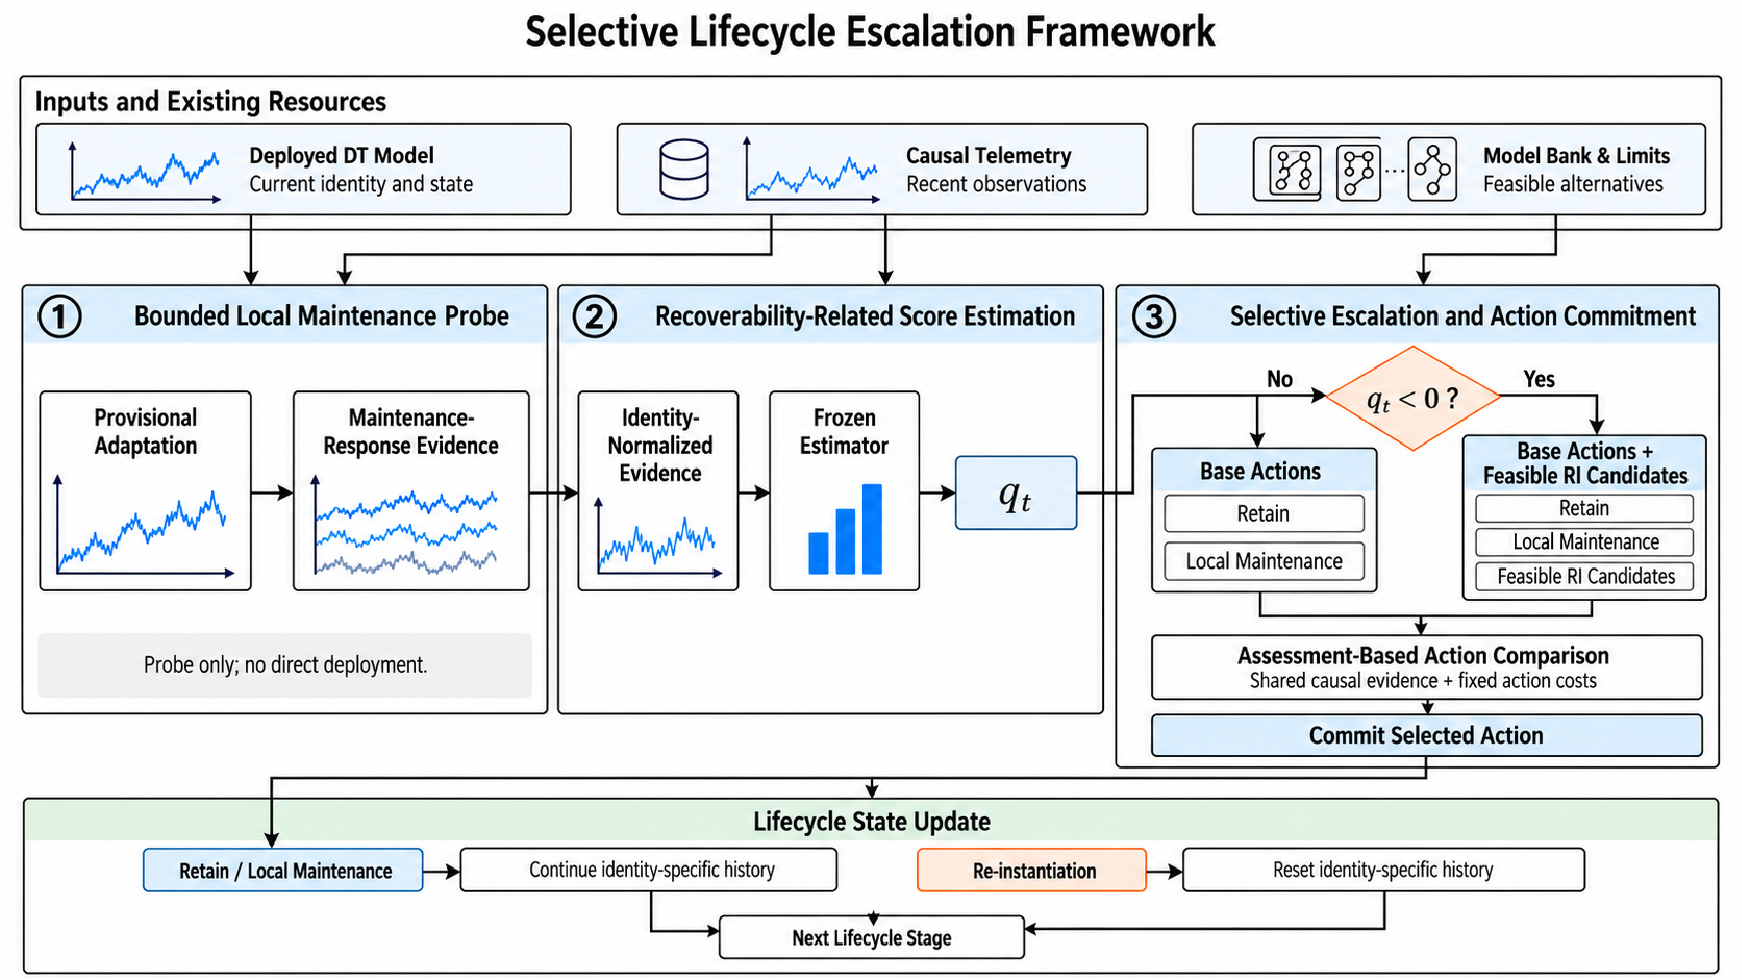
\includegraphics[width=0.99\textwidth]{figures/Fig1_Selective_Lifecycle_Escalation.pdf}
\caption{Selective lifecycle escalation with score-gated RI admission and action commitment.}
\label{fig:framework}
\end{figure*}
\section{Experimental Setup}
\subsection{Integrity-Correction Replication and Causal Stage Protocol}
The integrity-correction replication reuses 20 originally held-out,
subsequently observed synthetic computing centers (IDs 33000--33019),
three seeds (7311, 7312, and 7313), four frozen scenarios (C0, C1,
C3, and C4), and five lifecycle strategies. Each
center--seed--scenario--method combination forms a separate 24-stage
trajectory, yielding 1200 trajectories and 28,800 stage records.
The corrected evaluation uses one verified, ordered 20-center
batch-generation realization (F1) shared across all methods; it is
not a new, previously unseen held-out evaluation.
\par\noindent\textbf{Scenario construction.}
Base traces use a fixed data seed and heterogeneous monitoring configurations; the common intervention starts at raw observation 6520 (stage-9 assessment). C0 retains the native target and telemetry without an added regime intervention. C1 applies a gradual target-logit shift rising from zero to 0.8 over 5120 observations, with channel-specific delayed telemetry responses. C3 abruptly permutes and recalibrates telemetry channels and reverses target-logit deviations around the center-specific base logit. C4 retains telemetry but replaces targets according to a fixed multi-lag rule with a nonlinear interaction. Thus, C3 changes \emph{both} monitored inputs and target behavior; C4 is a changed target-generating mechanism, not merely added noise. These synthetic mechanisms are not a proof of external generalization.
 The five methods are compared under shared exogenous scenario inputs,
starting-state references, model-bank identities, and deployment limits
within each center--seed--scenario group.

The initial timeline reserves 800 raw observations for warm-up and
200 subsequent observations for the first identity-reference scale.
At stage $t$, the assessment segment begins at raw index
$b_t=1400+640(t-1)$. The update, assessment, and service segments
span $[b_t-400,b_t)$, $[b_t,b_t+240)$, and
$[b_t+240,b_t+640)$, respectively. Update and assessment data
are accessible before action selection; the service segment is
exposed to the online controller only after the selected action is
committed and sealed. Each segment is windowed within its own role
using a 96-observation input context, yielding 304 update, 144
assessment, and 304 service prediction targets, respectively.
From the second stage onward, the update segment reuses the preceding
stage's service observations; these are past data at the new decision,
not future information. Stage-level service loss is evaluated on the
committed model state.

The estimator and feature scaler, model-bank checkpoints, candidate
feasibility rules, admission boundary, action penalties, and analysis
protocol remained frozen for the integrity correction. The original
1200-record inventory combined 239 full-batch and 961 singleton
materializations, including one cross-method input mismatch. After
that discrepancy was identified, the correction used a verified common
batch20 input bundle for all methods, without pooling old trajectories
into the replication. The completed replication independently certifies
1200 unique trajectories, all 240 five-method groups, 60 shared initial
references, and their stage-level input and deployment-condition parity.
The original results and execution evidence remain preserved.
No estimator refitting, threshold retuning, model-bank change, or
population reselection was performed. The controlled runtime used
pandas 2.3.3, River 0.23.0, and psutil 7.2.2; full numerical
equivalence to the historical runtime is not certified.

\subsection{Compared Methods}
Table~\ref{tab:methods} summarizes the five compared lifecycle
strategies. The always-open comparator exposes model-level
alternatives at every stage but does not force their commitment.

\begin{table}[!b]
\caption{Compared Lifecycle Strategies}
\label{tab:methods}
\centering
\footnotesize
\begin{tabular}{p{0.12\columnwidth}p{0.78\columnwidth}}
\toprule
Method & Lifecycle behavior \\
\midrule
B0 & Frozen deployed model; no maintenance or re-instantiation. \\
B1 & Unconditional 50-update fixed-identity maintenance at every stage. \\
B2 & Five-block local candidate with recent and historical validation; no RI. \\
B8 & Model-level candidate search is always admissible; actions remain subject to comparison. \\
Proposed & Score-gated model-level search; $q_t<0$ admits alternatives but does not force re-instantiation. \\
\bottomrule
\end{tabular}
\end{table}

\noindent\textbf{B2 verification rule.} B2 forms its deployable local candidate by partitioning the 304 update-window examples into five blocks and independently adapting a copy of the current parent for 10 updates per block. It averages the five parameter deltas (the frozen $\beta=0.1$ produces zero actually trimmed blocks) and uses six assessment error-difference blocks plus bounded historical evidence to decide whether to commit. The recent median-plus-$0.5$-MAD must not exceed $-0.000028018231776243602$, and the historical median must not exceed zero; otherwise B2 retains the parent. B2 never admits RI. The common 50-update probe is also executed but is not the B2 deployable block candidate; thus B2's online path includes 50 probe updates plus 50 block-candidate updates. Its logged local-action penalty does not enter the B2 verification acceptance condition.


\subsection{Endpoints and Statistical Analysis}
The primary endpoint is \emph{mean lifecycle service loss}, measured
as post-commit service mean squared error (MSE). Service loss is
averaged over the 24 stages of each trajectory, then over seeds and
scenarios within a center, and finally over the 20 centers.
For each proposed-minus-baseline contrast, the observed point estimate
is the difference of center-aggregated method means.
Marginal percentile 95\% confidence intervals use 4000 paired
center-level bootstrap resamples with a shared center-index matrix
(seed 2904), maintaining method pairing within each resample.
The resampled mean difference is not substituted for the observed
point estimate. These four marginal intervals do not guarantee
simultaneous family-wise coverage. Scenario-stratified analysis is
reported separately. No additional unseen evaluation population
was sampled after the original results became available.

Secondary measures include retain, local-maintenance,
re-instantiation, and model-level-search admission rates, together
with recorded feasible-candidate counts, candidate-search optimizer
updates, and attributed decision-runtime measurements. The reported
action-cost measure sums frozen penalties for \emph{committed}
local-maintenance and re-instantiation actions; it excludes mandatory
probes, unselected candidate adaptations, and estimator inference.
Search-workload counters and attributed timers are descriptive and
must not be interpreted as complete end-to-end computational cost.
No post-hoc weighted composite endpoint is introduced.

For offline decision diagnostics, the frozen common service
threshold is
$\tau_{\mathrm{final}}=0.003039302364413743$.
After each online action is sealed, a finite-policy hindsight
reference $R_t^{\mathrm{fin}}(\tau_{\mathrm{final}})$ is computed from
the pre-decision model identity and future service segments as
specified in Section~IV-B. This threshold differs from the
center--seed-specific $\tau_{\mathrm{fit}}$ used for estimator
supervision and is not used to calibrate $q_t$ or to change the
operational rule $q_t<0$. Offline labels support all-stage
summaries of retain and escalation outcomes over 5760 proposed-method
decisions; they are not inputs to online action selection and must
not be interpreted as an online classifier-accuracy measure.
\begin{figure*}[!t]
\centering
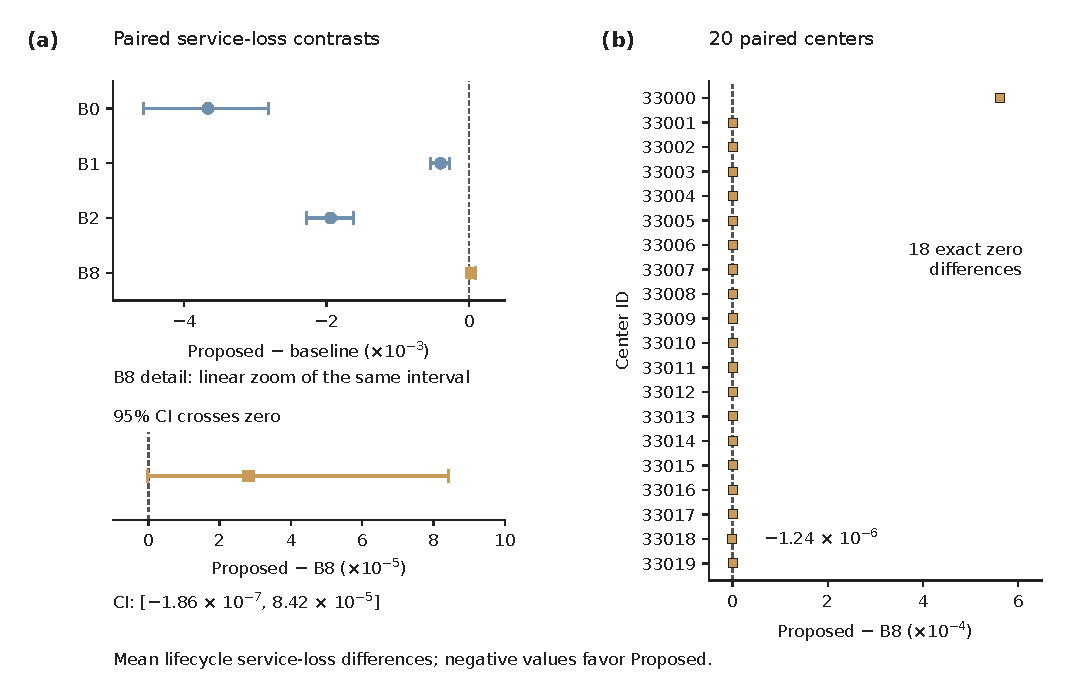
\includegraphics[width=0.96\textwidth]{figures/Fig2_Paired_Service_Loss.pdf}
\caption{Paired service-loss contrasts and center-level Proposed--B8 differences.}
\label{fig:paired-loss}
\end{figure*}
\section{Results and Analysis}
\subsection{Primary Lifecycle Service Loss}
Table~\ref{tab:main} reports the corrected, fully paired batch20
replication. The proposed policy achieves lower mean lifecycle service
loss than B0, B1, and B2, with the respective marginal 95\% paired
center-bootstrap intervals entirely below zero. Its observed loss is
slightly higher than B8, but the interval for that comparison crosses
zero. The evidence therefore establishes neither superiority,
noninferiority, nor equivalence relative to always-open search.

\begin{table*}[t]
\caption{Corrected Batch20 Mean Lifecycle Service Loss and Paired Comparisons}
\label{tab:main}
\centering
\footnotesize
\begin{tabular}{lccc}
\toprule
Method & Mean lifecycle service loss & Observed Proposed $-$ baseline & Marginal 95\% paired center-bootstrap CI \\
\midrule
B0 & 0.006604799 & $-0.003664155$ & [$-0.004573828$, $-0.002813402$] \\
B1 & 0.003341980 & $-0.000401336$ & [$-0.000543519$, $-0.000273248$] \\
B2 & 0.004883941 & $-0.001943298$ & [$-0.002280026$, $-0.001616486$] \\
B8 & 0.002912627 & $+0.000028017$ & [$-1.86\times10^{-7}$, $+8.42\times10^{-5}$] \\
Proposed & 0.002940644 & -- & -- \\
\bottomrule
\end{tabular}
\end{table*}



The observed differences use the original center-aggregated method
means rather than bootstrap replicate means. The shared-resample
index matrix contains 4000 draws of 20 center indices (seed 2904).
Figure~\ref{fig:paired-loss} visualizes the paired contrasts and center-level
Proposed--B8 differences. In the saved center-aggregated records,
18 of 20 centers show exactly zero Proposed--B8 difference; the
remaining differences are concentrated in two centers. This is a
descriptive observation, not evidence of statistical equivalence or
identical actions at all lifecycle stages. The B8 interval narrowly
extends below zero; failure to separate methods by this interval is
not an equivalence test. These are integrity-correction replication
estimates from previously observed synthetic centers, not evidence
from a newly unseen test population.

\begin{figure*}[!t]
\centering
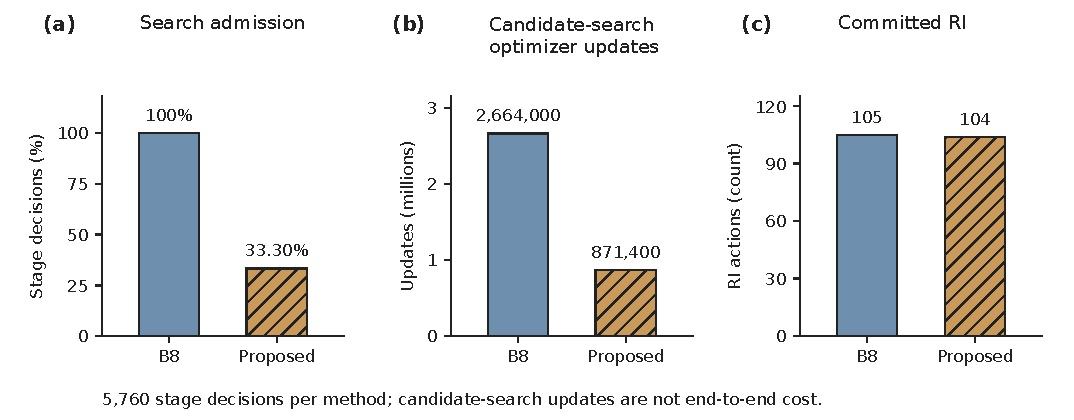
\includegraphics[width=0.935\textwidth]{figures/Fig3_Selective_Search.pdf}
\caption{Search admission, candidate-search updates, and committed RI actions.}
\label{fig:selective-search}
\end{figure*}
\subsection{Selective Search and Action Use}
Table~\ref{tab:actions} reports committed action frequencies and
penalties; Fig.~\ref{fig:selective-search} contrasts model-level search
with final RI commitment. B8 admits search at every stage; the proposed
policy admits it at 33.30\% of stages (1918 of 5760). Their observed
RI counts are 105 and 104, respectively, corresponding to 1.82\% and
1.81\% of stages. Thus, search admission does not itself imply an
identity transition, and similar overall RI counts do not establish
identical switching times or identities.

\begin{table*}[t]
\caption{Committed Actions, Model-Level Admission, and Action Penalties}
\label{tab:actions}
\centering
\footnotesize
\begin{tabular}{lrrrrr}
\toprule
Method & Maintenance rate & RI rate & Action penalty & Retain rate & Gate-open rate \\
\midrule
B0 & 0 & 0 & 0 & 1.0000 & 0 \\
B1 & 1.0000 & 0 & 0.00583546 & 0 & 0 \\
B2 & 0.2887 & 0 & 0.00168479 & 0.7113 & 0 \\
B8 & 0.1240 & 0.01823 & 0.00178711 & 0.8578 & 1.0000 \\
Proposed & 0.1259 & 0.01806 & 0.00178812 & 0.8561 & 0.3330 \\
\bottomrule
\end{tabular}
\end{table*}



Figure~\ref{fig:selective-search} separates model-level search
admission, candidate-search optimizer updates, and committed RI
actions. B8 and Proposed record 2,664,000 and 871,400 candidate-search
updates, respectively (67.29\% fewer for Proposed), and 105 versus
104 committed RI actions. Their recorded feasible candidate counts
are 53,280 and 17,428. Attributed decision-runtime totals are
34,281 and 15,102 seconds, respectively, but include implementation
and resource-scheduling effects rather than isolated end-to-end
computational costs. Committed-action penalties also exclude
mandatory probes, unselected candidate adaptations, and estimator
inference. Reduced search does not establish that every omitted
search was unnecessary.

\subsection{Scenario-Stratified Behavior}
Table~\ref{tab:scenario} compares Proposed and B8 under the four
frozen scenarios. Their C0 mean service losses coincide in the saved
results. Proposed has a slightly lower C1 observed mean, whereas B8
has lower C3 and C4 means. Scenario means alone do not establish
statistical equivalence or a significant scenario-specific difference.
The gate remains selective in every scenario, but this does not
imply uniformly better service outcomes.

\begin{table}[t]
\caption{Scenario-Stratified Proposed and B8 Results}
\label{tab:scenario}
\centering
\footnotesize
\begin{tabular}{lrrrr}
\toprule
Scenario & B8 loss & Proposed loss & Gate-open & RI rate \\
\midrule
C0 & 0.00284816 & 0.00284816 & 0.4090 & 0 \\
C1 & 0.00267605 & 0.00266895 & 0.2743 & 0 \\
C3 & 0.00331095 & 0.00342327 & 0.3375 & 0.04375 \\
C4 & 0.00281535 & 0.00282220 & 0.3111 & 0.02847 \\
\bottomrule
\end{tabular}
\end{table}

\subsection{Offline Decision Diagnostics}
The corrected offline diagnostic inventory covers 5760 proposed-method
stage decisions: 407 correct-retain events, 12 unnecessary-RI events,
92 correct-escalation events, and 2100 missed-escalation flags.
These named labels neither exhaust all stages nor form a complete
classifier confusion matrix. Specifically, a missed-escalation flag
means that RI was not committed while the finite fixed-identity
hindsight recoverability margin was negative. It does not establish
that a deployment-feasible RI candidate would have won assessment-based
action comparison, nor that the admission gate was necessarily closed.

The substantial missed-escalation count limits claims about precise
switching-time identification and full-class unrecoverability. These
finite-reference labels were computed offline, after online decisions,
and did not enter the online admission rule.

\FloatBarrier
\section{Discussion}
\subsection{Interpretation of Selective Escalation}
Model-level search admission and RI commitment remain distinct.
The recoverability-related score $q_t$ admits model-level alternatives
to assessment-based action comparison, but that comparison may still
retain the incumbent or select fixed-identity maintenance. In the
corrected replication, the gate admits search at 33.30\% of stages
while recording nearly the same number of RI commitments as B8.
This does not establish identical switching times or identities.

The observed service-loss difference to B8 is small, and its marginal
95\% interval crosses zero. This permits neither a superiority claim
nor the stronger conclusion of equivalence or noninferiority. The
measured candidate-search update count is substantially lower under
selective admission, supporting reduced model-level search work under
the recorded protocol. Attributed decision timers do not establish a
full end-to-end computational advantage; action penalties cover only
committed actions. The method therefore demonstrates a restricted
search--service trade-off rather than uniform optimality.

\subsection{Limits of Recoverability Evidence and Generalization}
The theoretical quantity $\mathcal R_t^M$ is defined over a causal
class of bounded fixed-identity maintenance policies. By contrast,
the implemented offline reference evaluates four one-shot maintenance
choices with fixed parameters over a finite future-service horizon.
A negative margin over this subset cannot certify full-class
unrecoverability. The frozen estimator regresses identity-normalized
finite-policy targets using center--seed-specific fitting thresholds,
and its score is not recalibrated to the common threshold used for
offline diagnostics. The rule $q_t<0$ is an admission heuristic,
not a certified horizon-level failure of current-identity maintenance.

The correction addressed a material cross-method pairing failure in
the original mixed-context run. Its uniform batch20 inputs, shared
initial states and deployment conditions are certified, but the
population had already been observed when this integrity-correction
replication was undertaken. Numerical equivalence to the entire
historical software environment remains unverified, and stochastic
outcomes are not claimed to be bitwise invariant under all worker
schedules. These boundaries do not invalidate the corrected paired
comparison, but they preclude presenting it as a new unseen holdout
or a perfect replay of every historical execution condition.

The large number of finite-reference missed-escalation flags limits
claims about switching-time identification: a flag does not prove
that RI would have been the best feasible action at that stage.
The experiments further cover synthetic centers, four specified
scenarios and a fixed model bank; they do not establish cross-domain
deployment or complete computational cost. Future work should assess
prospective score calibration, multi-stage maintenance references,
and full-cost behavior on external traces while preserving the
causal split between online decisions and hindsight diagnostics.
\section{Conclusion}
This paper examined when continued fixed-identity maintenance of a
deployed digital-twin model may be insufficient and model-level
alternatives should be considered. We defined bounded fixed-identity
maintenance recoverability and developed a frozen admission estimator
supervised by finite one-shot maintenance references, without claiming
to solve the full theoretical policy-class optimization. The resulting
score conditionally admits deployment-feasible model-level candidates
to an assessment-based comparison with retention and local maintenance.
In a corrected replication on 20 previously evaluated synthetic
centers, the proposed policy achieved lower mean lifecycle service
loss than three fixed-identity baselines and opened model-level search
at 33.30\% of stages, with 67.29\% fewer candidate-search updates than
always-open search. Relative to always-open search, the observed
service-loss difference was small and its marginal 95\% interval
crossed zero; neither equivalence nor noninferiority was established.
Substantial offline missed-escalation flags and the synthetic,
post-observation evaluation scope limit claims about exact RI timing
and broader generalization. Future work should evaluate prospective
score calibration, multi-stage maintenance evidence and end-to-end
costs on independent external traces.
% Ordered by first citation in main.tex; generated from verified metadata.
\begin{thebibliography}{99}
\bibitem{Sharma2022} Angira Sharma, Edward Kosasih, Jie Zhang, Alexandra Brintrup, Anisoara Calinescu, ``Digital Twins: State of the Art Theory and Practice, Challenges, and Open Research Questions,'' \emph{Journal of Industrial Information Integration}, vol. 30, pp. 100383, 2022. DOI: \href{https://doi.org/10.1016/j.jii.2022.100383}{10.1016/j.jii.2022.100383}.
\bibitem{Mihai2022} Stefan Mihai, Mahnoor Yaqoob, Dang V. Hung, et al., ``Digital Twins: A Survey on Enabling Technologies, Challenges, Trends and Future Prospects,'' \emph{IEEE Communications Surveys and Tutorials}, vol. 24, 2022. DOI: \href{https://doi.org/10.1109/COMST.2022.3208773}{10.1109/COMST.2022.3208773}.
\bibitem{Xu2023} Hansong Xu, Jun Wu, Qianqian Pan, Xinping Guan, Mohsen Guizani, ``A Survey on Digital Twin for Industrial Internet of Things: Applications, Technologies and Tools,'' \emph{IEEE Communications Surveys and Tutorials}, vol. 25, pp. 2569--2598, 2023. DOI: \href{https://doi.org/10.1109/COMST.2023.3297395}{10.1109/COMST.2023.3297395}.
\bibitem{Tang2022} Fengxiao Tang, Xuehan Chen, Tiago Koketsu Rodrigues, Ming Zhao, Nei Kato, ``Survey on Digital Twin Edge Networks (DITEN) Toward 6G,'' \emph{IEEE Open Journal of the Communications Society}, vol. 3, pp. 1360--1381, 2022. DOI: \href{https://doi.org/10.1109/OJCOMS.2022.3197811}{10.1109/OJCOMS.2022.3197811}.
\bibitem{Qin2024} Baolin Qin, Heng Pan, Yueyue Dai, et al., ``Machine and Deep Learning for Digital Twin Networks: A Survey,'' \emph{IEEE Internet of Things Journal}, vol. 11, pp. 34694--34716, 2024. DOI: \href{https://doi.org/10.1109/JIOT.2024.3416733}{10.1109/JIOT.2024.3416733}.
\bibitem{Tao2026} Ming Tao, Lingling Liao, Yin Zhang, et al., ``EDT-SaFL: Semi-Asynchronous Federated Learning for Edge Digital Twin in Industrial Internet-of-Things,'' \emph{IEEE Transactions on Mobile Computing}, vol. 25, pp. 674--690, 2026. DOI: \href{https://doi.org/10.1109/TMC.2025.3595117}{10.1109/TMC.2025.3595117}.
\bibitem{Luo2025} Tianxiang Luo, Hui Zhang, Haotong Cao, Tamer Mohamed Abdellatif, Sherif Moussa, ``Enabling Real-Time Digital Twin in Social IoT System Through Personalized Federated Learning,'' \emph{IEEE Internet of Things Journal}, vol. 12, pp. 35037--35047, 2025. DOI: \href{https://doi.org/10.1109/JIOT.2025.3590746}{10.1109/JIOT.2025.3590746}.
\bibitem{Wang2024CL} Liyuan Wang, Xingxing Zhang, Hang Su, Jun Zhu, ``A Comprehensive Survey of Continual Learning: Theory, Method and Application,'' \emph{IEEE Transactions on Pattern Analysis and Machine Intelligence}, vol. 46, pp. 5362--5383, 2024. DOI: \href{https://doi.org/10.1109/TPAMI.2024.3367329}{10.1109/TPAMI.2024.3367329}.
\bibitem{Zhang2023OneNet} Yi-Fan Zhang, Qingsong Wen, Xue Wang, et al., ``OneNet: Enhancing Time Series Forecasting Models under Concept Drift by Online Ensembling,'' \emph{Advances in Neural Information Processing Systems}, vol. 36, pp. 69949--69980, 2023. DOI: \href{https://doi.org/10.52202/075280-3066}{10.52202/075280-3066}.
\bibitem{Kim2022RevIN} Taesung Kim, Jinhee Kim, Yunwon Tae, Cheonbok Park, Jang-Ho Choi, Jaegul Choo, ``Reversible Instance Normalization for Accurate Time-Series Forecasting Against Distribution Shift,'' \emph{International Conference on Learning Representations}, 2022. \href{https://mlanthology.org/iclr/2022/kim2022iclr-reversible/}{[Online]}.
\bibitem{Liu2022NST} Yong Liu, Haixu Wu, Jianmin Wang, Mingsheng Long, ``Non-stationary Transformers: Exploring the Stationarity in Time Series Forecasting,'' \emph{Advances in Neural Information Processing Systems}, vol. 35, 2022. DOI: \href{https://doi.org/10.52202/068431-0718}{10.52202/068431-0718}.
\bibitem{Wang2022CoTTA} Qin Wang, Olga Fink, Luc Van Gool, Dengxin Dai, ``Continual Test-Time Domain Adaptation,'' \emph{Proceedings of the IEEE/CVF Conference on Computer Vision and Pattern Recognition}, pp. 7201--7211, 2022. \href{https://openaccess.thecvf.com/content/CVPR2022/html/Wang_Continual_Test-Time_Domain_Adaptation_CVPR_2022_paper.html}{[Online]}.
\bibitem{Niu2022EATA} Shuaicheng Niu, Jiaxiang Wu, Yifan Zhang, et al., ``Efficient Test-Time Model Adaptation without Forgetting,'' \emph{Proceedings of the 39th International Conference on Machine Learning}, vol. 162, pp. 16888--16905, 2022. \href{https://proceedings.mlr.press/v162/niu22a.html}{[Online]}.
\bibitem{Yuan2023RoTTA} Longhui Yuan, Binhui Xie, Shuang Li, ``Robust Test-Time Adaptation in Dynamic Scenarios,'' \emph{Proceedings of the IEEE/CVF Conference on Computer Vision and Pattern Recognition}, pp. 15922--15932, 2023. \href{https://openaccess.thecvf.com/content/CVPR2023/html/Yuan_Robust_Test-Time_Adaptation_in_Dynamic_Scenarios_CVPR_2023_paper.html}{[Online]}.
\bibitem{Song2023EcoTTA} Junha Song, Jungsoo Lee, In So Kweon, Sungha Choi, ``EcoTTA: Memory-Efficient Continual Test-Time Adaptation via Self-Distilled Regularization,'' \emph{Proceedings of the IEEE/CVF Conference on Computer Vision and Pattern Recognition}, pp. 11920--11929, 2023. \href{https://openaccess.thecvf.com/content/CVPR2023/html/Song_EcoTTA_Memory-Efficient_Continual_Test-Time_Adaptation_via_Self-Distilled_Regularization_CVPR_2023_paper.html}{[Online]}.
\bibitem{Niu2023SAR} Shuaicheng Niu, Jiaxiang Wu, Yifan Zhang, et al., ``Towards Stable Test-Time Adaptation in Dynamic Wild World,'' \emph{International Conference on Learning Representations}, 2023. \href{https://mlanthology.org/iclr/2023/niu2023iclr-stable/}{[Online]}.
\bibitem{Liu2024MAE} Jiaming Liu, Ran Xu, Senqiao Yang, et al., ``Continual-MAE: Adaptive Distribution Masked Autoencoders for Continual Test-Time Adaptation,'' \emph{Proceedings of the IEEE/CVF Conference on Computer Vision and Pattern Recognition}, pp. 28653--28663, 2024. \href{https://openaccess.thecvf.com/content/CVPR2024/html/Liu_Continual-MAE_Adaptive_Distribution_Masked_Autoencoders_for_Continual_Test-Time_Adaptation_CVPR_2024_paper.html}{[Online]}.
\bibitem{Yang2024CTTA} Xu Yang, Xuan Chen, Moqi Li, Kun Wei, Cheng Deng, ``A Versatile Framework for Continual Test-Time Domain Adaptation: Balancing Discriminability and Generalizability,'' \emph{Proceedings of the IEEE/CVF Conference on Computer Vision and Pattern Recognition}, pp. 23731--23740, 2024. \href{https://openaccess.thecvf.com/content/CVPR2024/html/Yang_A_Versatile_Framework_for_Continual_Test-Time_Domain_Adaptation_Balancing_Discriminability_CVPR_2024_paper.html}{[Online]}.
\bibitem{Chen2024VPTTA} Ziyang Chen, Yongsheng Pan, Yiwen Ye, Mengkang Lu, Yong Xia, ``Each Test Image Deserves A Specific Prompt: Continual Test-Time Adaptation for 2D Medical Image Segmentation,'' \emph{Proceedings of the IEEE/CVF Conference on Computer Vision and Pattern Recognition}, pp. 11184--11193, 2024. \href{https://openaccess.thecvf.com/content/CVPR2024/html/Chen_Each_Test_Image_Deserves_A_Specific_Prompt_Continual_Test-Time_Adaptation_CVPR_2024_paper.html}{[Online]}.
\bibitem{Nie2023PatchTST} Yuqi Nie, Nam H. Nguyen, Phanwadee Sinthong, Jayant Kalagnanam, ``A Time Series Is Worth 64 Words: Long-Term Forecasting with Transformers,'' \emph{International Conference on Learning Representations}, 2023. \href{https://mlanthology.org/iclr/2023/nie2023iclr-time/}{[Online]}.
\bibitem{Wang2024EndEdge} Yingchao Wang, Chen Yang, Shulin Lan, Liehuang Zhu, Yan Zhang, ``End-Edge-Cloud Collaborative Computing for Deep Learning: A Comprehensive Survey,'' \emph{IEEE Communications Surveys and Tutorials}, vol. 26, pp. 2647--2683, 2024. DOI: \href{https://doi.org/10.1109/COMST.2024.3393230}{10.1109/COMST.2024.3393230}.
\bibitem{Li2022EfficientFormer} Yanyu Li, Geng Yuan, Yang Wen, et al., ``EfficientFormer: Vision Transformers at MobileNet Speed,'' \emph{Advances in Neural Information Processing Systems}, vol. 35, 2022. DOI: \href{https://doi.org/10.52202/068431-0940}{10.52202/068431-0940}.
\bibitem{Li2023EfficientFormerV2} Yanyu Li, Ju Hu, Yang Wen, et al., ``Rethinking Vision Transformers for MobileNet Size and Speed,'' \emph{Proceedings of the IEEE/CVF International Conference on Computer Vision}, pp. 16889--16900, 2023. \href{https://openaccess.thecvf.com/content/ICCV2023/html/Li_Rethinking_Vision_Transformers_for_MobileNet_Size_and_Speed_ICCV_2023_paper.html}{[Online]}.
\bibitem{Lin2021MCUNetV2} Ji Lin, Wei-Ming Chen, Han Cai, Chuang Gan, Song Han, ``MCUNetV2: Memory-Efficient Patch-based Inference for Tiny Deep Learning,'' \emph{Advances in Neural Information Processing Systems}, vol. 34, 2021. \href{https://proceedings.neurips.cc/paper_files/paper/2021/file/1371bccec2447b5aa6d96d2a540fb401-Paper.pdf}{[Online]}.
\end{thebibliography}

\end{document}
